% -*- root: ../../DAT2-A423_Project_Report.tex -*-

\begin{infobox}{\section[A Study of the JPEG file format]{A Study of the JPEG file format\footnotenomarker{This section may be omitted without loss of continuity}}}

\subsection*{An Overview of JPEG}
JPEG is an image format defined by the Joint Photographic Experts Group. 
This type of image requires much more computing power to process, both in terms of encoding and decoding, compared to a much more simple format like Windows BMP, this will become more clear in the following sections. 
A crucial thing to note about JPEG is that one of the things that allows the image to be compressed, is that the encoding process is lossless, which means that when saving an image to JPEG, you lose information about the individual pixels.

\subsection*{JPEG as a file format}

JPEG has a very comprehensive standard, which defines the inner workings of the JPEG compression. 
What this standard does not describe however, is an actual file format \citep{Miano1999}. 
The standard does not define how to encode images in a way, such that all JPEG encoders can decode the image. 
An example of this is, that the standard does not define how colours are represented in the format, which means that one decoder could potentially use a RGB colour space while another one would use a RBG space, both systems are perfectly valid according to the JPEG standard.

Without a way to ensure that all decoders would read an encoded image the same way, an image file isn't worth much. This is why the JPEG File Interchange Format specification \citep{JFIFSpecs} was developed by Eric Hamilton. JFIF defines a standard which all JPEG files must abide. This standard includes a definition of the colour being encoded in one or three channels. One channel if it is a monochrome image, and three channels if it is a true-colour image. If encoded in three channels, the colour space used is YCbCr, if only one channel is used only the luminance (Y) channel is used.

The JFIF specification is what allows JPEG images to be as widespread as they are today, where JPEG are used by large services like Facebook to store and serve small images of reasonable quality.

[Et eller andet introværk]

\subsection*{The Process of Encoding a JFIF Image}
When encoding a JFIF image, we start off with a Bitmap, that is, a two dimensional array of pixels each consisting of a R, G and B value. The first step is transforming those colour channels into the colour space used in JFIF images. 

\subsubsection*{The Colour-space}
When describing colours in terms of computer science, we often use the colour space RGB, where each component corresponds to the intensity of the red, blue and green LEDs that make up a pixel on our screen. A colour in the YCbCr colour system is made up from the luminance (Y) which describes light intensity together with the blue-difference and the red-difference chroma components which together describes the actual colour.

When converting from RGB to YCbCr we can use matrix multiplication, and find the Y, Cb and Cr components as a matrix product:

$$\begin{bmatrix}
	Y\\Cb\\Cr
\end{bmatrix} = \begin{bmatrix}
	0.299 & 0.587 & 0.144\\
	-0.1687 & -0.3313 & 0.5\\
	0.5 & -0.4187 & -0.0813
\end{bmatrix}\begin{bmatrix}
	R\\G\\B
\end{bmatrix}$$

Likewise, we can calculate the R, G and B components from the YCbCr colour space:

$$\begin{bmatrix}
	R\\G\\B
\end{bmatrix} = \begin{bmatrix*}[l]
	Y&+&1.402 &\cdot & (Cr-128)&\\
	Y &-& 0.34414&\cdot &(Cb-128) &- &0.71414&\cdot&(Cr-128)\\
	Y &+& 1.772&\cdot& (Cb-128)&
\end{bmatrix*}$$

These values all range from 0 to 255, like the R, G and B values. However when we later will encode these values, it is much more efficient to have them centered around 0 instead, so that the values range from -128 to 127. To do this, we simple subtract 128 from each Y, Cb and Cr value. 

\subsubsection*{Sampling}
When looking at an image, the eye is much more sensitive to small changes in the luminance channels, than they are to changes in the chroma channels. Luckily, we can use this fact to compress our image even more in terms of filesize using a technique called sampling. 

The JPEG standard allows each component to be sampled. This means that we can use sampling to scale each component individually. In reality, we calculate luminance for every pixel in the image, while only calculating the chroma channels for each 2x2 block. This gives us a sampling of 2x2 for the luminance component, while the chroma components have a sampling of 1x1. This means that for every 1 pixel in the x direction we calculate the chroma components, we calculate 2 luminance components, and the same with the y direction. Put in another way, we have 4 times as much information about the luminance component than of the chroma components.

\begin{centering}
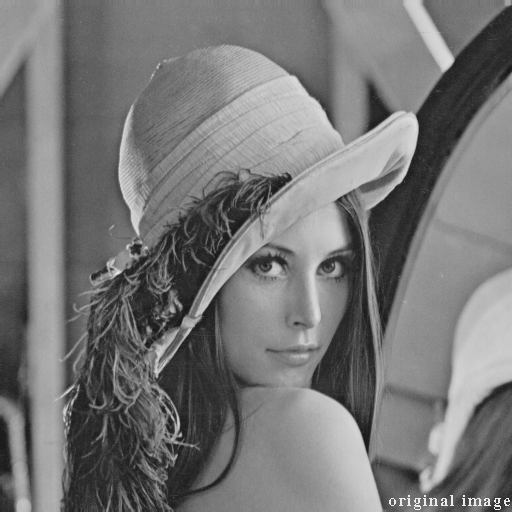
\includegraphics[width=.4\linewidth]{lenaYchannel.png}
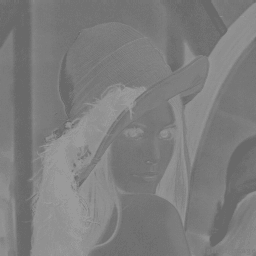
\includegraphics[width=.2\linewidth]{lenaCbchannel.png}
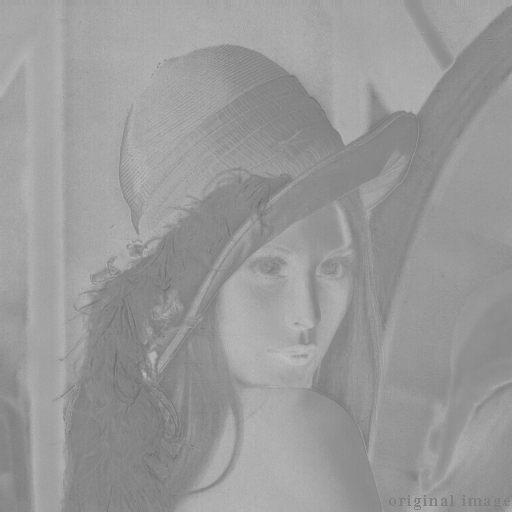
\includegraphics[width=.2\linewidth]{lenaCrchannel.png}
\captionof{figure}{Y, Cb and Cr Channels of an Image}\label{fig:YCbCrChannels}
\end{centering}

\subsubsection*{Discrete Cosine Transform}
After sampling the image, it must be split into blocks called MCU's. The default size of an MCU is 8x8 pixel, but it changes when sampling is used. In the section above, we used a sampling of 4:2:0 where the chroma channels where downscaled by 50\% in both directions. This means that when the sampling of 4:2:0 is used, we have a MCU of size 16x16 pixels.

For each 8x8 block of pixels in our MCU's we perform DCT. The two dimensional DCT is given by:

$$ G_{u,v} = c(u,v)\sum_{x=0}^{7}\sum_{y=0}^{7}g_{x,y}\cos{\left(\frac{(2x+1)u\pi}{16}\right)}\cos{\left(\frac{(2y+1)v\pi}{16}\right)} $$

where:
\begin{itemize}
	\item $u$ is the horizontal spatial frequency 
	\item $v$ is the vertical spatial frequency 
	\item $c(u,v) = \begin{cases}\frac{1}{8} \quad \quad \quad \quad\text{if } u=v=0\\ 
	                             0.17677 \quad \text{ if } u = 0 \text{ or } v = 0\\
	                             \frac{1}{4} \quad \quad \quad \quad\text{otherwise}
	                             \end{cases} $
    \item $g_{x,y}$ is the value of pixel at coordinates $(x,y)$ 
\end{itemize}

\subsubsection*{Quantization}
Quantization tables are what makes JPEG compression lossy. 
After the DTC process, the quantization progress are performed on the resulting 8x8 block of values.  
Quantization is the process of dividing each value in the 8x8 block with a corresponding value in a quantization table. 
The JPEG specification allows 4[SOURCE NEEDED, JEG ER IKKE SIKKER] quantization tables to be used, while JFIF limits it even further to 2 tables. 
This means that two of our three channels have to share quantization tables. 
As the retina in the eye are much more sensible to changes in the luminance channel, JFIF specifies that the luminance channel gets it own quantization table, while the chroma components must share a quantization table.

Although the JPEG standard does not force you to use default tables, they do provide some tables which has shown good results with their test images. The proposed quantization table for the image channels are shown below.

\begin{centering}
\hspace{-3mm}\tcbox[left=0mm,right=0mm,top=0mm,bottom=0mm,boxsep=0mm,
toptitle=0.5mm,center title, bottomtitle=0.5mm,nobeforeafter,title=Proposed Quantization Table for Luminance Channel]{
\small
	 	\begin{tabular}{|c|c|c|c|c|c|c|c|}\hline
			16 & 11 & 10 & 16 & 24 & 40 & 51 & 61 \\ \hline
			12 & 12 & 14 & 19 & 26 & 58 & 60 & 55 \\ \hline
			15 & 14 & 16 & 24 & 40 & 57 & 69 & 56 \\ \hline
			14 & 17 & 22 & 29 & 51 & 87 & 80 & 62 \\ \hline
			18 & 24 & 37 & 56 & 68 & 109 & 103 & 77 \\ \hline
			24 & 35 & 55 & 64 & 81 & 104 & 113 & 92 \\ \hline
			49 & 64 & 78 & 87 & 103 & 121 & 120 & 101 \\ \hline
			72 & 92 & 95 & 98 & 112 & 100 & 103 & 99 \\ \hline
		\end{tabular}
}
\tcbox[left=0mm,right=0mm,top=0mm,bottom=0mm,boxsep=0mm,
toptitle=0.5mm,center title, nobeforeafter,bottomtitle=0.5mm,title=Proposed Quantization Table for Chroma Channels]{
\small
	 	\begin{tabular}{|c|c|c|c|c|c|c|c|}\hline
			17 & 18 & 24 & 47 & 99 & 99 & 99 & 99\\ \hline
			18 & 21 & 26 & 66 & 99 & 99 & 99 & 99\\ \hline
			24 & 26 & 56 & 99 & 99 & 99 & 99 & 99\\ \hline
			47 & 66 & 99 & 99 & 99 & 99 & 99 & 99\\ \hline
			99 & 99 & 99 & 99 & 99 & 99 & 99 & 99\\ \hline
			99 & 99 & 99 & 99 & 99 & 99 & 99 & 99\\ \hline
			99 & 99 & 99 & 99 & 99 & 99 & 99 & 99\\ \hline
			99 & 99 & 99 & 99 & 99 & 99 & 99 & 99\\ \hline
		\end{tabular}
}
\end{centering}

\subsection*{Dissection of a JPEG file}
\subsubsection*{Segments in a JPEG file}
\begin{wraptable}{r}{5.5cm}
\caption{Most commonly used markers in JPEG files}
\label{tab:markers}
\begin{tabular}{|p{2.7cm}|l|}
\hline
Marker & Identifier\\ \hline
0xFFD8 & SOI\\ \hline
0xFFE$n$ \newline$(n = \{0 \ldots F\})$ & APP$n$\\ \hline
0xFFD8 & DQT \\ \hline
0xFFC0 & SOF \\ \hline
0xFFC4 & DHT\\ \hline
0xFFDA & SOS\\ \hline
0xFFD9 & EOI\\ \hline 
\end{tabular}
\end{wraptable}

The JPEG standard defines that a JPEG file must be ordered in segments. These segments are each indicator by a marker, and the most common segment markers are shown in table \ref{tab:markers}. Most of the markers are followed by 2 bytes of data describing the length of the following segment. Knowing the length makes it possible for a decoder to skip segments it does not know how to understand. 

As is shown by table \ref{tab:markers}, all markers start with the byte 0xFF, there exists one special case, where 0xFF does not define a marker, and that case is if the following byte is 0x00. More on this later, when it is examined how image data is written to a file.

\subsubsection*{The SOI and EOI markers}
\begin{centering}
\hspace{1.2cm}\tcbox[left=0mm,right=0mm,top=0mm,bottom=0mm,boxsep=0mm,
toptitle=0.5mm,center title, nobeforeafter, bottomtitle=0.5mm,title=Start of Image (SOI) Segment]{
	 	\begin{tabular}{|l|l|l|}
			Size in bytes  & Description \\ \hline \hline
			2 bytes  & SOI marker\\ \hline
		\end{tabular}
} \tcbox[left=0mm,right=0mm,top=0mm,bottom=0mm,boxsep=0mm,
toptitle=0.5mm,center title, nobeforeafter,bottomtitle=0.5mm,title=End of Image (EOI) Segment]{
	 	\begin{tabular}{|l|l|l|}
			Size in bytes  & Description \\ \hline \hline
			2 bytes  & EOI marker\\ \hline
		\end{tabular}
}
\end{centering}\\
The first marker a JPEG decoder meets in a JPEG file is the SOI (Start of Image) marker. The marker does not specify a length in the following bytes, since the segment only consists of the marker itself. Likewise, the last marker a decoder will meet is the EOI (End of Image) marker, which specifies that all data has been read from the image.

\subsubsection*{The APP$n$ marker}
\begin{centering}
\tcbox[left=0mm,right=0mm,top=0mm,bottom=0mm,boxsep=0mm,
toptitle=0.5mm,center title, bottomtitle=0.5mm,title=APP$n$ Segment]{
	 	\begin{tabular}{|l|l|l|}
			Size in bytes  & Description \\ \hline \hline
			2 bytes  & APP$n$ marker\\ \hline
			2 bytes & Segment length\\ \hline
			variable & Application specific data
		\end{tabular}
}
\end{centering}
The JPEG standard defines the APP segments to be application specific data, which can be placed anywhere in the image file. Applications can then use these segments to store additional information about the image file. JFIF specifies that the APP$_0$ is used for identifying the file as a valid JFIF file, and that the APP$_0$ segment must be placed immediately after the SOI marker.

By convention the APP$n$ segments use a null terminated string for identifying themselves. The JFIF APP segment as found in almost all JPEG files can be seen in table \ref{JFIFAPP0}.

\begin{centering}
\tcbox[left=0mm,right=0mm,top=0mm,bottom=0mm,boxsep=0mm,
toptitle=0.5mm,center title, bottomtitle=0.5mm,title=JFIF APP$_0$ Segment]{

	 	\begin{tabular}{|l|l|l|}
			Size in bytes  & Value \\ \hline \hline
			2 bytes  & APP$_0$ marker\\ \hline
			2 bytes & Segment length\\ \hline
			5 bytes & Null terminated string ``JFIF''\\ \hline
			2 bytes & Major and minor version number\\ \hline
			1 byte & Units for setting photo density\\ \hline
			4 bytes & X-density and Y-density\\ \hline
			2 bytes & Width and height of thumbnail image\\ \hline
			variable & Thumbnail data saved in RGB colour space.\\ \hline
		\end{tabular}
}

	 	\captionof{table}{JFIF APP$_0$ Segment}\label{JFIFAPP0}
\end{centering}

\subsubsection*{The DQT marker}
\begin{centering}
\tcbox[left=0mm,right=0mm,top=0mm,bottom=0mm,boxsep=0mm,
toptitle=0.5mm,center title, bottomtitle=0.5mm,title=Define Quantization Table Segment]{
	 	\begin{tabular}{|l|l|l|}
			Size in bytes  & Description \\ \hline \hline
			2 byte  & DQT marker\\ \hline
			4 bits & Quantization value size (0 = 1 byte, 1 = 2 bytes) \\ \hline
			4 bits & Table identifier (0-3) \\ \hline
			64 or 128 bytes & Unsigned quantization values\\ \hline
		\end{tabular}
}
\end{centering}



\end{infobox}